\documentclass[tikz]{standalone}

\usetikzlibrary{automata}

\begin{document}
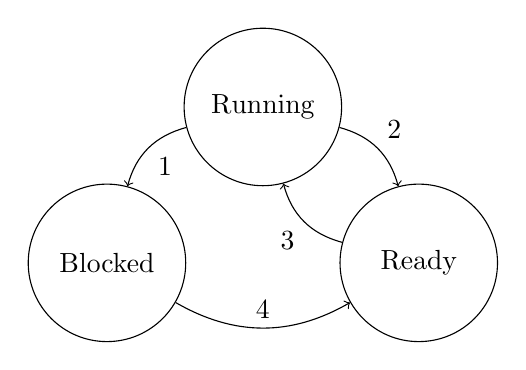
\begin{tikzpicture}
	[auto,node distance=2.8cm,]
	\tikzstyle{state}=[circle, draw, minimum size=2cm];

	\node[state] (A) {Running};
	\node[state] (B) [below right of=A] {Ready};
	\node[state] (C) [below left of=A] {Blocked};

	\path
	(A) edge[->,bend right] node {1} (C)
	(C) edge[->,bend right] node {4} (B)
	(B) edge[->,bend left] node {3} (A)
	(A) edge[->,bend left] node {2} (B);

\end{tikzpicture}
\end{document}